% Created 2020-05-02 Sat 13:44
% Intended LaTeX compiler: pdflatex
\documentclass[11pt]{article}
\usepackage[utf8]{inputenc}
\usepackage[T1]{fontenc}
\usepackage{graphicx}
\usepackage{grffile}
\usepackage{longtable}
\usepackage{wrapfig}
\usepackage{rotating}
\usepackage[normalem]{ulem}
\usepackage{amsmath}
\usepackage{textcomp}
\usepackage{amssymb}
\usepackage{capt-of}
\usepackage{hyperref}
\usepackage[a4paper,margin=20mm]{geometry}
\usepackage{amsmath}
\usepackage{amsfonts}
\usepackage{bm}
\newcommand{\tr}{\textsf{T}}
\newcommand{\grad}{\bm{\nabla}}
\newcommand{\av}[2][]{\mathbb{E}_{#1\!}\left[ #2 \right]}
\newcommand{\Prob}[2][]{\mathbb{P}_{#1\!}\left[ #2 \right]}
\newcommand{\logg}[1]{\log\!\left( \strut#1 \right)}
\newcommand{\e}[1]{{\rm e}^{#1}}
\newcommand{\dd}{\mathrm{d}}
\DeclareMathAlphabet{\mat}{OT1}{cmss}{bx}{n}
\newcommand{\normal}[2]{\mathcal{N}\!\left(#1 \big| #2 \right)}
\newcounter{eqCounter}
\newcommand{\beq}{\setcounter{eqCounter}{0}}
\newcommand{\eq}[1][=]{\stepcounter{eqCounter}\stackrel{\text{\tiny(\arabic{eqCounter})}}{#1}}
\author{Adam Prügel-Bennett}
\date{\today}
\title{Advanced Machine Learning Subsidary Notes\\\medskip
\large Lecture 18: Generative Models}
\hypersetup{
 pdfauthor={Adam Prügel-Bennett},
 pdftitle={Advanced Machine Learning Subsidary Notes},
 pdfkeywords={},
 pdfsubject={},
 pdfcreator={Emacs 26.3 (Org mode 9.1.9)}, 
 pdflang={English}}
\begin{document}

\maketitle



\section{Keywords}
\label{sec:orgc04738f}
\begin{itemize}
\item Generative models, graphical models, LDA
\end{itemize}

\section{Main Points}
\label{sec:org4ac7d34}

\subsection{Bayesian Inference}
\label{sec:orga60037f}
\begin{itemize}
\item Most Bayesian inference involves constructing a model of the
underlying data generation process and  using Bayes' rule to
learn unknown properties of the model
\item In building models we use random variables, \(X\), \(Y\), \(Z\),
etc. to model quantities we are uncertain about
\item We associate \emph{probability mass functions} \(\Prob{X,Y,Z}\) (for
discrete random variable) or \emph{probability densities}
\(f_{X,Y,Z}(x,y,z)\) (for continuous random variables)
\item Often our tasks will be to infer these probability distributions
(or parameters of these probability distribution) for quantities
of interest
\item In classical machine learning we may think the feature vector
\(\bm{X}\) as being a random variable and the prediction \(Y\) as
being a second random variable
\item \textbf{Discriminative Models}
\begin{itemize}
\item Often our goal is to learn the probability distribution \(\Prob{Y|\bm{X}}\)
\item Very often we would parameterise this distribution with some
parameters \(\bm{\Theta}\) and our task would be to learn these
parameters based on training data
\end{itemize}
\item \textbf{Generative Models}
\begin{itemize}
\item Surprisingly it is  often easier to model the joint probability
\(\Prob{Y,\bm{X}}\)
\item This means that we model the process of both generating the
targets and the feature vectors together
\item These are known as \emph{generative models} as they allow us to
generate random examples
\item We don't necessary want to use them to generate random samples
it just makes the modelling process easier (although you need
to get used to this as it feel counter-intuitive)
\item we can use generative models to do discrimination
\item Examples of generative models include \emph{Hidden Markov Models}
and \emph{Topic Models} (covered later)
\end{itemize}
\item \textbf{Latent Variables}
\begin{itemize}
\item In building probabilistic models we often model quite
complicated processes
\item To do this we often introduce intermediate processes
\item This leads to introduce other random variables that we actually
never observe
\item These are known as \textbf{latent variable}
\item Often our model will involve many different layers between the
inputs \(\bm{X}\) and targets \(Y\): this process is sometimes
known as \emph{hierarchical  modelling}
\end{itemize}
\item \textbf{Mixtures of Gaussians}
\begin{itemize}
\item To illustrate latent variables and a simple hierarchical model
we consider a classic probabilistic model known as \emph{mixture of Gaussians}
\item We consider a concrete scenario
\item We suppose we are observing the decay of two types (\(A\) and
\(B\)) of short-lived particles
\item We can measure their half lives, \(X_i\), but we don't know the type
of particle
\item We have a measurement error of the half-life
\item Let \(Z_i \in \{0,1\}\) equal 1 if  particle \(i\) is of type \(A\)
and 0 if it is of type \(B\)
\item The probability distribution of the half-life measurement is
therefore
$$ f(X_i|Z_i,\bm{\Theta}) = Z_i\,\normal{X_i}{\mu_A,\sigma_A^2} +
         (1-Z_i)\,\normal{X_i}{\mu_B,\sigma_B^2} $$
\begin{itemize}
\item where \(\mu_A\) and \(\mu_B\) are the expected half-lives for
particles of type \(A\) and \(B\) respectively
\item \(\sigma_A\) and \(\sigma_B\) are the standard deviations in the measurements
\item this just says that if the \(i^{th}\) particle is of type \(A\)
then the probability of \(X_i\) is
\(\normal{X_i}{\mu_A,\sigma_A^2}\) and if it is of type \(B\) it
is \(\normal{X_i}{\mu_B,\sigma_B^2}\)
\end{itemize}
\item We assume that we have \(m\) observations (e.g. \(m=1\,000\))
\begin{figure}[htbp]
\centering
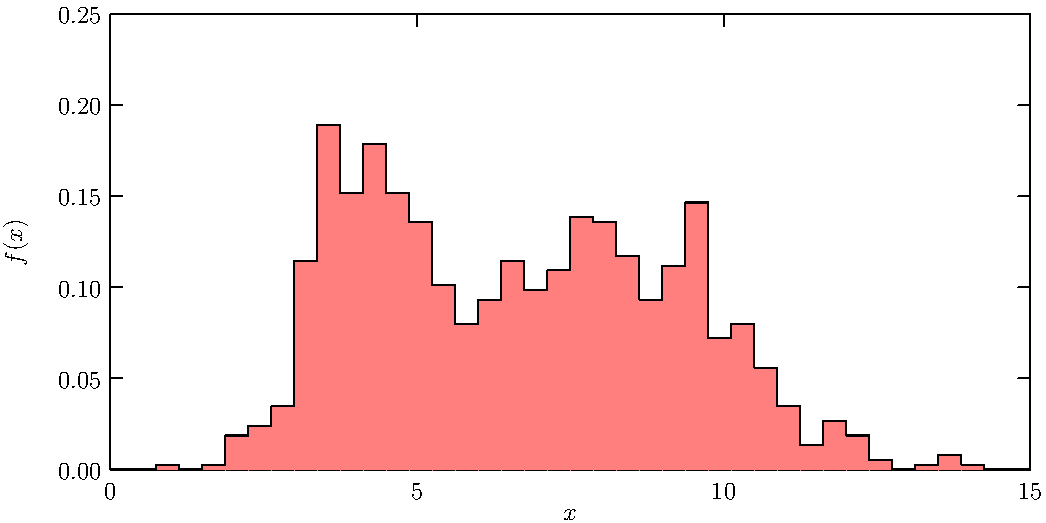
\includegraphics[width=0.6\textwidth]{./figures/mixtureOfGaussiansData.pdf}
\caption{Example of distribution of half-lives}
\end{figure}
\item Our job is to infer the random variables \(\bm{\Theta}=(\mu_1,
       \mu_2, \sigma_1, \sigma_2, p)\), where \(p=\Prob{Z_i=1}\) is the
probability of the particle being type \(A\)
\item We can do a full Bayesian calculation, but let us just use a
maximum likelihood
\item The maximum likelihood of the data
\(\mathcal{D}=\{X_i|i=1,2,\ldots,m\}\) is
\begin{align*}\beq
f(\mathcal{D}|\bm{\Theta}) 
&\eq \sum_{\bm{Z}\in\{0,1\}^m}  f(\mathcal{D},\bm{Z}|\bm{\Theta}) \\
&\eq \prod_{i=1}^m \sum_{Z_i\in\{0,1\}} f(X_i, Z_i | \bm{\Theta})
\eq \prod_{i=1}^m  \sum_{Z_i\in\{0,1\}}
f(X_i | Z_i, \bm{\Theta}) \, \Prob{Z_i}
\end{align*}
\begin{enumerate}
\item where we marginalise out the latent variables
\(\bm{Z}=(Z_1,Z_2,\ldots Z_n)\)
\item we assume the data is independent
\item we use the identity \(f(X_i, Z_i | \bm{\Theta})= f(X_i | Z_i, \bm{\Theta}) \, \Prob{Z_i}\)
\end{enumerate}
\item It is usually easier working with the log-likelihood
\begin{align*}
\logg{f(\mathcal{D}|\bm{\Theta})} &= \sum_{i=1}^m
\logg{\strut f(X_i|Z_i=1) \, \Prob{Z_i=1} + f(X_i|Z_i=0) \,
\Prob{Z_i=0} }\\
 &=\sum_{i=1}^m
\logg{p\,\normal{X_i}{\mu_A,\sigma_A}+(1-p)\,\normal{X_i}{\mu_B,\sigma_B}}
\end{align*}
\item We could do gradient descent on this, but it is an ugly
expression to work with
\end{itemize}
\item \textbf{Expectation Maximisation}
\begin{itemize}
\item Rather than maximise the likelihood directly we iteratively
maximise the expected log-likelihood starting form some guess
\(\bm{\Theta}^{(0)}\) we get an improved guess
$$ \bm{\Theta}^{(t+1)} = \mathop{\mathrm{argmax}}_{\bm{\Theta}}
       \sum_{\bm{Z}\in\{0,1\}^m} \Prob{\bm{Z}\middle|\mathcal{D},\bm{\Theta}^{(t)}}\,
       \logg{f(\mathcal{D},\bm{Z} | \bm{\Theta})} $$
\item This is a general optimisation strategy that is regularly used
when we have latent variables
\item It is known as \textbf{expectation maximisation} or the \textbf{EM-algorithm}
\item This looks very different to maximising the log-likelihood: it
takes some effort to understand why this works
\item To understand this we note
$$f(\mathcal{D},\bm{Z}|\bm{\Theta}) =
       f(\mathcal{D}|\bm{Z},\bm{\Theta}) \, \Prob{\bm{Z}|\bm{\Theta}}  $$
From which we can deduce
$$ \logg{f(\mathcal{D}|\bm{\Theta})} = \logg{f(\mathcal{D},\bm{Z}|\bm{\Theta})} - \logg{\Prob{\bm{Z}|\bm{\Theta}} } $$
\item We now consider the probability distribution
\(\Prob{\bm{Z}\middle|\mathcal{D},\bm{\Theta}^{(t)}}\), that
tells us the probability that \(Z_i=1\) given \(X_i\) and the
parameters \(\bm{\Theta}^{(t)}\)
\item If we not take expectations of
\(\logg{f(\mathcal{D}|\bm{\Theta})}\) give above with respect to
this distribution then
\begin{align*}
  \logg{f(\mathcal{D}|\bm{\Theta})}
   &= \av[\bm{Z}|\bm{\Theta}^{(t)}]{\logg{f(\mathcal{D},\bm{Z}|\bm{\Theta})}}
- \av[\bm{Z}|\bm{\Theta}^{(t)}]{\logg{\Prob{\bm{Z}|\bm{\Theta}} }}
  \\
  &= Q(\bm{\Theta}|\bm{\Theta}^{(t)}) +
  S(\bm{\Theta}|\bm{\Theta}^{(t)})
\end{align*}
\begin{itemize}
\item Note that the left-hand side does not involve the latent
variables so when we take the expectation we get itself
\item The first term on the right-hand side is
$$ Q(\bm{\Theta}|\bm{\Theta}^{(t)}) =
         \av[\bm{Z}|\bm{\Theta}^{(t)}]{\logg{f(\mathcal{D},\bm{Z}|\bm{\Theta})}}
	 =  \sum_{\bm{Z}\in\{0,1\}^m} \Prob{\bm{Z}\middle|\mathcal{D},\bm{\Theta}^{(t)}}\,
         \logg{f(\mathcal{D}|\bm{Z}, \bm{\Theta})} $$
\item This is the term we are optimising in \emph{expectation maximisation}
\item The second term is
$$ S(\bm{\Theta}|\bm{\Theta}^{(t)}) = - \av[\bm{Z}|\bm{\Theta}^{(t)}]{\logg{\Prob{\bm{Z}|\bm{\Theta}} }}
	 =  - \sum_{\bm{Z}\in\{0,1\}^m} \Prob{\bm{Z}\middle|\mathcal{D},\bm{\Theta}^{(t)}}\,
         \logg{\Prob{\bm{Z}|\bm{\Theta}}} $$
\end{itemize}
\item Using the identity for the log-likelihood we can write the
change in log-likelihood when we update our
parameters 
\begin{align*}
\Delta f &=
\logg{f(\mathcal{D}|\bm{\Theta}^{(t+1)})} -
\logg{f(\mathcal{D}|\bm{\Theta}^{(t)})} \\
&= Q(\bm{\Theta}^{(t+1)}|\bm{\Theta}^{(t)}) -
Q(\bm{\Theta}^{(t)}|\bm{\Theta}^{(t)})
+ S(\bm{\Theta}^{(t+1)}|\bm{\Theta}^{(t)}) -
S(\bm{\Theta}^{(t)}|\bm{\Theta}^{(t)}) \\
&= Q(\bm{\Theta}^{(t+1)}|\bm{\Theta}^{(t)}) -
Q(\bm{\Theta}^{(t)}|\bm{\Theta}^{(t)})
+ \mathrm{KL}\!\left( \Prob{\bm{Z}|\bm{\Theta}^{(t)}} \middle\|
  \Prob{\bm{Z}|\bm{\Theta}^{(t+1)}} \right)
 \end{align*}
\begin{itemize}
\item where
\end{itemize}
\begin{align*}
\mathrm{KL}\!\left( \Prob{\bm{Z}|\bm{\Theta}^{(t)}} \middle\|
\Prob{\bm{Z}|\bm{\Theta}^{(t+1)}} \right) &=
S(\bm{\Theta}^{(t+1)}|\bm{\Theta}^{(t)}) -
S(\bm{\Theta}^{(t)}|\bm{\Theta}^{(t)}) \\
&= -  \sum_{\bm{Z}\in\{0,1\}^m} \Prob{\bm{Z}\middle|\mathcal{D},\bm{\Theta}^{(t)}}\,
\logg{\frac{ \Prob{\bm{Z}|\bm{\Theta}^{(t+1)}} }{ \Prob{\bm{Z}|\bm{\Theta}^{(t)}} }} 
\end{align*}
\begin{itemize}
\item We shown in a previous lecture that KL-divergences are non-negative
\end{itemize}
\item Now in expectation maximisation we choose
$$ \bm{\Theta}^{(t+1)} = \mathop{\mathrm{argmax}}_{\bm{\Theta}}
       Q(\bm{\Theta}|\bm{\Theta}^{(t)}) $$
which implies \(Q(\bm{\Theta}^{(t+1)}|\bm{\Theta}^{(t)}) \geq
       Q(\bm{\Theta}^{(t)}|\bm{\Theta}^{(t)})\)
\item Thus \(\Delta f\geq 0\)
\item This gives us a relative simple procedure we need to maximise
$$ Q(\bm{\Theta}|\bm{\Theta}^{(t)}) = \sum_{\bm{Z}\in\{0,1\}^m} \Prob{\bm{Z}\middle|\mathcal{D},\bm{\Theta}^{(t)}}\,
       \logg{f(\mathcal{D}|\bm{Z}, \bm{\Theta})} $$
\item Let us return to the problem of working out the half-life statistics of
our two types of particles \(A\) and \(B\)
\item Recall \(f(\mathcal{D},\bm{Z} |\bm{\Theta}) =
       \prod\limits_{i=1}^m  f(X_i|Z_i,\bm{\Theta}) \, \Prob{Z_i}\) where
$$ f(X_i,Z_i|\bm{\Theta}) = p\, Z_i\,\normal{X_i}{\mu_A,\sigma_A^2} +
         (1-p)\,(1-Z_i)\,\normal{X_i}{\mu_B,\sigma_B^2} $$
\item Let 
 \begin{align*}
 p_i^{(t)} &= \Prob{Z_i=1\middle|X_i, \bm{\Theta}^{(t)}} = 
 \frac{p^{(t)}\, \normal{X_i}{\mu_A^{(t)},\sigma_A^{2(t)}} }
{ p^{(t)}\,\normal{X_i}{\mu_A^{(t)},\sigma_A^{2(t)}} + (1-p^{(t)})\, \normal{X_i}{\mu_B^{(t)},\sigma_B^{2(t)}} } \\
 q_i^{(t)} &= \Prob{Z_i=0\middle|X_i, \bm{\Theta}^{(t)}} =
 \frac{(1-p^{(t)})\,\normal{X_i}{\mu_B^{(t)},\sigma_B^{2(t)}}}
{p^{(t)}\, \normal{X_i}{\mu_A^{(t)},\sigma_A^{2(t)}} + (1-p^{(t)})\, \normal{X_i}{\mu_B^{(t)},\sigma_B^{2(t)}} }
 = 1-p_i^{(t)}
 \end{align*}
\item Then
\begin{align*}
Q(\bm{\Theta}|\bm{\Theta}^{(t)}) &= \sum_{i=1}^m \;
p_i^{(t)} \logg{p^{(t)}\,\normal{X_i}{\mu_A,\sigma_A^{2}}}
+ q_i^{(t)}  \logg{(1-p^{(t)})\,\normal{X_i}{\mu_B,\sigma_B^{2}}} \\ 
&= \sum_{i=1}^m \;
p_i^{(t)}\left(\log(p) -
\frac{(X_i-\mu_A)^2}{2\sigma_A^{2}}
  - \frac{1}{2} \logg{2\,\pi\,\sigma_A^{2}} \right) \\
  &\hspace{1cm}
  + q_i^{(t)}\left(\log(1-p) -
  \frac{(X_i-\mu_B)^2}{2\sigma_B^{2}}
  - \frac{1}{2} \logg{2\,\pi\,\sigma_B^{2}} \right) 
  \end{align*}
\item To optimise this we just set the derivatives to 0
\begin{itemize}
\item Optimising with respect to \(p\)
$$ \frac{\partial Q(\bm{\Theta}|\bm{\Theta}^{(t)})}{\partial p}
           = \frac{1}{p} \sum_{i=1}^m \; p_i^{(t)} - \frac{1}{1-p}
           \sum_{i=1}^m \; q_i^{(t)} =0 $$
solving for \(p\)
$$ p^{(t+1)} = \frac{\sum\limits_{i=1}^m 
          p_i^{(t)}}{\sum\limits_{i=1}^m (p_i^{(t)}+q_i^{(t)})} =
          \frac{1}{m} \sum\limits_{i=1}^m  p_i^{(t)}$$
\item Optimising with respect to \(\mu_A\)
$$ \frac{\partial Q(\bm{\Theta}|\bm{\Theta}^{(t)})}{\partial \mu_A} 
	 = - \sum\limits_{i=1}^m p_i^{(t)} \frac{X_i-\mu_A}{\sigma_A^{2}} $$
solving for \(\mu_A\) (and performing a similar optimisation
for \(\mu_B\))
$$ \mu_A^{(t+1)} = \frac{ \sum\limits_{i=1}^m
         p_i^{(t)} X_i }{\sum\limits_{i=1}^m p_i^{(t)}} ,\quad\quad
	 \mu_B^{(t+1)} = \frac{ \sum\limits_{i=1}^m
         q_i^{(t)} X_i }{\sum\limits_{i=1}^m q_i^{(t)}} $$
\item Putting in the optimal value for \(\mu^{(t)}_A\) and optimising with respect to \(\sigma_A^2\)
 $$ \frac{\partial Q(\bm{\Theta}|\bm{\Theta}^{(t)})}{\partial \sigma^2_A}
	  = \frac{1}{2\,\sigma^4_A}\sum_{i=1}^m p_i^{(t)}
          (X_i-\mu^{(t)}_A)^2- \frac{1}{\sigma_A^{2}}\sum_{i=1}^m p_i^{(t)}$$
Solving for \(\sigma^2_A\) (and performing a similar optimisation
for \(\sigma^2_B\))
$$ \sigma_A^2 = \frac{ \sum\limits_{i=1}^m
         p_i^{(t)} (X_i-\mu^{(t)}_A)^2 }{\sum\limits_{i=1}^m p_i^{(t)}}
         ,\quad\quad
	  \sigma_B^2 = \frac{ \sum\limits_{i=1}^m
         q_i^{(t)} (X_i-\mu^{(t)}_B)^2 }{\sum\limits_{i=1}^m q_i^{(t)}}$$
\end{itemize}
\item These are very natural update equations
\begin{itemize}
\item we make an estimate, \(p_i^{(t)\) of the probability that observation \(X_i\)
is a particle of type \(A\) or \(B\) base on our current parameters
\item we then update all our parameters based on these estimates
\end{itemize}
\item We are guaranteed that our EM-algorithm always involves an
improving step
\item For the data set we showed earlier (which was a random sample
of size 1000 generated using \(p=0.3\), \(\mu_A=4\),
\(\sigma_A=0.8\), \(\mu_B=8\) and \(\sigma_B=2\) we get the results
shown in figure \ref{fig:mog}
\begin{figure}[htbp]
\centering
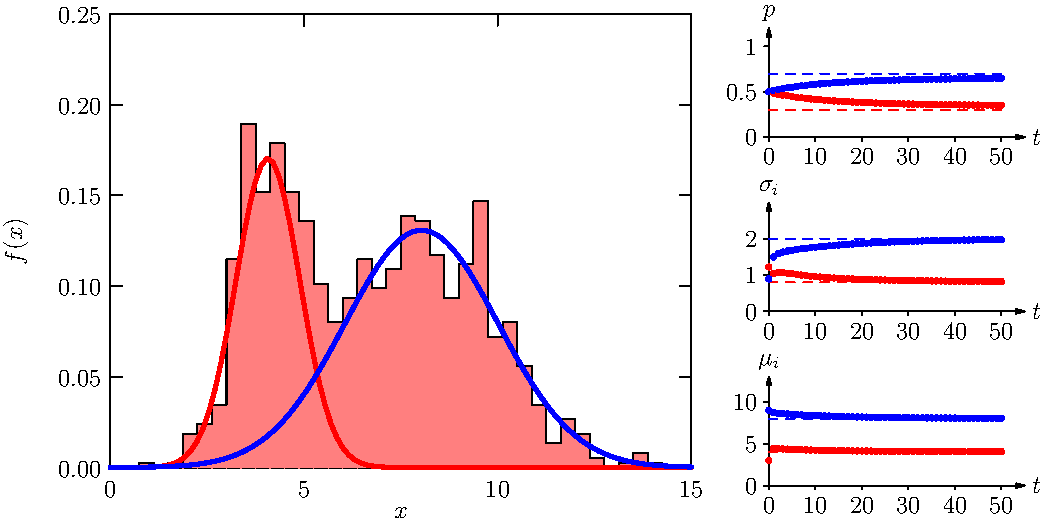
\includegraphics[width=0.8\textwidth]{./figures/mixtureOfGaussians-50.pdf}
\caption{Example of EM algorithm to compute the statistics for the half-lives of our two particles \label{fig:mog}}
\end{figure}
\end{itemize}
\end{itemize}

\section{Exercises}
\label{sec:orga759d75}

**

\section{Experiments}
\label{sec:orgcb61389}

**
\end{document}
